\PassOptionsToPackage{subsection=false}{beamerouterthememiniframes}
\PassOptionsToPackage{dvipsnames,table}{xcolor}
\documentclass[fleqn]{beamer}
\usepackage{graphicx}
\usepackage{multirow}
\usepackage{multicol}
\usepackage{amsmath,amsfonts,amsthm,amsopn}
\usepackage{color, colortbl}
\usepackage{subfig}
\usepackage{wrapfig}
\usepackage{fancybox}
\usepackage{tikz}
\usepackage{fancyhdr}
\usepackage{setspace}
\usepackage{xcolor}
\usepackage{movie15}
\usepackage{pifont}
\usepackage{soul}
\usepackage{fancyvrb,newverbs}
\usepackage{epsfig}
\usepackage{epstopdf}
\fvset{fontsize=\footnotesize}
\RecustomVerbatimEnvironment{verbatim}{Verbatim}{}

%\usepackage{fancybox}

\usetheme{Szeged}
\usecolortheme{default}

%\definecolor{links}{HTML}{2A1B81}
%\definecolor{links}{blue!20}
\hypersetup{colorlinks,linkcolor=,urlcolor=blue!80}

\setbeamertemplate{blocks}[rounded]
\setbeamercolor{block title}{bg=blue!40,fg=black}
\setbeamercolor{block body}{bg=blue!10}


\newenvironment<>{clicker}[1]{%
  \begin{actionenv}#2%
      \def\insertblocktitle{#1}%
      \par%
      \mode<presentation>{%
        \setbeamercolor{block title}{fg=white,bg=magenta}
       \setbeamercolor{block body}{fg=black,bg=magenta!10}
       \setbeamercolor{itemize item}{fg=magenta}
       \setbeamertemplate{itemize item}[triangle]
       \setbeamercolor{enumerate item}{fg=magenta}
     }%
      \usebeamertemplate{block begin}}
    {\par\usebeamertemplate{block end}\end{actionenv}}

%\newcommand{\bmp}{\begin{minipage}}
%\newcommand{\emp}{\end{minipage}}
%\newcommand{\blankcolumn}{\bmp{.05\textwidth}\hspace{0.50in} \emp}

\defbeamertemplate*{footline}{infolines theme}
{
  \leavevmode%
  \hbox{%
  \begin{beamercolorbox}[wd=.333333\paperwidth,ht=2.25ex,dp=1ex,left]{author in head/foot}%
    \usebeamerfont{author in head/foot}~~\insertshortinstitute: \insertshorttitle
  \end{beamercolorbox}%
  \begin{beamercolorbox}[wd=.67\paperwidth,ht=2.25ex,dp=1ex,right]{date in head/foot}%
    \usebeamerfont{date in head/foot}%\insertshortdate{}\hspace*{2em}
    \insertframenumber{} / \inserttotalframenumber\hspace*{2ex}
  \end{beamercolorbox}
  }%
  \vskip0pt%
}

\newcommand{\cmark}{\ding{51}}%
\newcommand{\xmark}{\ding{55}}%
\newcommand{\grp}{\textcolor{magenta}{Group Exercise}}
\newcommand{\grpc}{\textcolor{magenta}{Group Exercise, continued}}
\newcommand{\bsans}[1]{\underline{\hspace{0.2in}\color{blue!80}{#1}\hspace{0.2in}}}

\definecolor{cverbbg}{gray}{0.93}
\newenvironment{cverbatim}
 {\SaveVerbatim{cverb}}
 {\endSaveVerbatim
  \flushleft\fboxrule=0pt\fboxsep=.5em
  \colorbox{cverbbg}{\BUseVerbatim{cverb}}%
  \endflushleft
}
\newenvironment{lcverbatim}
 {\SaveVerbatim{cverb}}
 {\endSaveVerbatim
  \flushleft\fboxrule=0pt\fboxsep=.5em
  \colorbox{cverbbg}{%
    \makebox[\dimexpr\linewidth-2\fboxsep][l]{\BUseVerbatim{cverb}}%
  }
  \endflushleft
}

\newcommand{\bmp}{\begin{minipage}}
\newcommand{\emp}{\end{minipage}}
\newcommand{\blankcolumn}{\bmp{.05\textwidth}\hspace{0.50in} \emp}

 \newenvironment{code}[1]%
  {\vspace{.1in}\footnotesize\Verbatim[frame=single,label=SAS Code,commandchars=\\\{\},xrightmargin=#1\textwidth,framesep=.2in,labelposition=all]}
  {\endVerbatim\normalsize}

 \newenvironment{Rcode}[1]%
  {\vspace{.1in}\footnotesize\Verbatim[frame=single,label=R Code,commandchars=\\\{\},xrightmargin=#1\textwidth,framesep=.2in,labelposition=all]}
  {\endVerbatim\normalsize}

   \newenvironment{RcodeScript}[1]%
  {\vspace{.1in}\scriptsize\Verbatim[frame=single,label=R Code,commandchars=\\\{\},xrightmargin=#1\textwidth,framesep=.2in,labelposition=all]}
  {\endVerbatim\normalsize}

 \newenvironment{RcodeTiny}[1]%
  {\vspace{.1in}\tiny\Verbatim[frame=single,label=R Code,commandchars=\\\{\},xrightmargin=#1\textwidth,framesep=.2in,labelposition=all]}
  {\endVerbatim\normalsize}


   \newenvironment{Rout}[1]%
  {\vspace{.1in}\footnotesize\Verbatim[frame=single,label=R Output,commandchars=\\\{\},xrightmargin=#1\textwidth,framesep=.2in,labelposition=all]}
  {\endVerbatim\normalsize}
  
     \newenvironment{MTout}[1]%
  {\vspace{.1in}\footnotesize\Verbatim[frame=single,label=Minitab Output,commandchars=\\\{\},xrightmargin=#1\textwidth,framesep=.2in,labelposition=all]}
  {\endVerbatim\normalsize}

   \newenvironment{RoutScript}[1]%
  {\vspace{.1in}\scriptsize\Verbatim[frame=single,label=R Output,commandchars=\\\{\},xrightmargin=#1\textwidth,framesep=.2in,labelposition=all]}
  {\endVerbatim\normalsize}

 \newenvironment{RoutTiny}[1]%
  {\vspace{.1in}\tiny\Verbatim[frame=single,label=R Output,commandchars=\\\{\},xrightmargin=#1\textwidth,framesep=.2in,labelposition=all]}
  {\endVerbatim\normalsize}

\newenvironment{craw}[2]%
{\vspace{.1in}\footnotesize\Verbatim[frame=single,label=#2,commandchars=\\\{\},xrightmargin=#1\textwidth,framesep=.2in,labelposition=all]}
  {\endVerbatim\normalsize}


\newenvironment{scriptcraw}[2]%
{\vspace{.1in}\scriptsize \Verbatim[frame=single,label=#2,commandchars=\\\{\},xrightmargin=#1\textwidth,framesep=.2in,labelposition=all]}
  {\endVerbatim\normalsize}

  \newenvironment{tinycraw}[2]%
{\vspace{.1in}\tiny \Verbatim[frame=single,label=#2,commandchars=\\\{\},xrightmargin=#1\textwidth,framesep=.2in,labelposition=all]}
  {\endVerbatim\normalsize}




\title[Set 1]{Introduction to Survival Analysis}
\author[Pileggi]{Shannon Pileggi}

\institute[STAT 417]{STAT 417}

\date{}


\begin{document}

\begin{frame}
\titlepage
\end{frame}

\begin{frame}
\frametitle{OUTLINE\qquad\qquad\qquad} \tableofcontents[hideallsubsections]
\end{frame}


%===========================================================================================================================
\section[Time to event data]{Characteristics of time to event data}
%===========================================================================================================================

\subsection{}

\begin{frame}
\frametitle{\grp}
\begin{clicker}{Survival analysis is statistical methodology only applied to the study of whether or not someone lives or dies.}
\begin{enumerate}
\item True
\item False
\end{enumerate}
\end{clicker}
%False!  Survival analysis is a field of statistics covering methods and techniques for examining and investigating time-to-event data.
\end{frame}

\begin{frame}
\frametitle{Chocolate chip activity}
\begin{itemize}
\item Outcome of interest:
\item[] %whether or not chip melts completely
\item[]
\item[]
\item Response variable of interest:
\item[] %time until chip melts (in seconds)
\item[]
\item[]
\item Noticeable feature(s) about the recorded values of the response variable:
\item[] %all positive  values
\item[] %some times are not "complete" (we know times until 80 seconds)
\item[]
\end{itemize}
\end{frame}

\begin{frame}
\frametitle{Survival data}
\begin{itemize}
\item The collection of lengths of times it takes for the chocolate chips to melt is an example of \textbf{survival data} (also called \textbf{time-to-event data} or \textbf{failure-time data}).
\item Time-to-event data are the times until the experimental (or observational) units experience a particular event
of interest.
\item Examples of events of interest:
\begin{enumerate}
\item %chip melts
\item %college graduation
\item %death from cancer
\item %re-arrest
\item %drug relapse
\end{enumerate}
\item Examples of units experiencing the event:
\begin{enumerate}
\item[] animate: %person, animal
\item[]
\item[] inanimate: %computer, light bulb
\item[]
\end{enumerate}
\end{itemize}
\end{frame}


\begin{frame}{Incomplete data}
Special features of survival data include \textbf{incomplete} data:
\begin{enumerate}
\item \textbf{Censoring}: Some event times may only partially known (the exact time until the event occurs is unknown)
\item \textbf{Truncation}: Certain subjects are excluded (screened) from the investigation due to some selection condition
\end{enumerate}
%\item Incomplete data create certain difficulties when trying to estimate basic descriptive quantities or when trying to fit models to the data.
%\item There are various categories of censoring and truncation to be discussed later.
\vskip10pt
\textbf{Note}: We'll refer to an exact known event time as \textbf{complete}.
\vskip10pt
\textbf{Chocolate chip example:}
\begin{itemize}
\item Some \emph{complete} melting times: %52, 53, 54, 79, 79
\item[]
\item Some \emph{censored} melting times: %at least 80 seconds
\item[]
\end{itemize}
\end{frame}

\begin{frame}
\frametitle{Survival time random variable}
The response variable of interest is the survival time random variable ($T$), also called the
\begin{itemize}
\item survival time
\item failure time
\item time-to-event random variable
\end{itemize}
\vskip20pt
$T = $
\vskip20pt
%the time until event random variable
%Value must be at least 0
The observed values of $T$ include \emph{both} the complete and censored survival times.
\end{frame}

\begin{frame}
\frametitle{\grp}
\begin{clicker}{Consider the chocolate chip activity.  Which of the following is the response variable for survival analysis?}
\begin{enumerate}
\item whether or not the chip is melted by 80 seconds
\item the time until the chocolate chip melts (seconds) %correct
\item the amount of the chip that is left over after 80 seconds
\item the time at which we stop monitoring the chip melting
\end{enumerate}
\end{clicker}
\end{frame}

\begin{frame}
\frametitle{Examples of time to event random variables}
\begin{enumerate}
\item Time until death after diagnosis of lung cancer (Medicine)
\item Age at which first alcoholic drink is taken (Public Health)
%\item Time until blocked drivers honk their horn (Psychology)
\item Time until students graduate from college (Education)
%\item Time until former inmates are rearrested (Criminology)
\item Other examples from your questionnaire:
\begin{itemize}
\item[]
\item %age at first bike ride (years)
\item[]
\item %time until first cell phone replacement (months)
\item[]
\item %time to get ready in the morning (minutes)
\item[]
\end{itemize}
\end{enumerate}
\end{frame}

\begin{frame}
\frametitle{Identify the time to event random variable}
\begin{enumerate}
\item \small{Diekmann et al. (1996) investigated the association between driver characteristics and social status of cars to aggressive driver responses by measuring the time that elapsed between the being blocked and honking the horn.}
\item[] $T=$
\item[] %time until motorist reacts aggressively (seconds)
\item \small{Hepburn (2005) found that the time to rearrest for drug-using criminal offenders depended on various socio-economic characteristics of the individual, as well as whether the drug-user was exposed to treatment.}
\item[] $T=$
\item[] %time until re-arrest from being released (months)
\item \small{Dickersin et al. (2002) investigated whether manuscripts submitted for publication in the \textit{Journal of the American Medical Association} that reported positive results from clinical trial studies were published more quickly than manuscripts reported negative results.}
\item[] $T=$
\item[] %time until submitted manuscript is published (months)
\end{enumerate}
\end{frame}


\begin{frame}
\frametitle{Research questions addressed}
\begin{itemize}
\item \small{What proportion of subjects will take longer than a particular time to experience an event of interest, i.e. survive beyond a certain time?}
%survival function (parametric or nonparametric)
\item[]
\item \small{What is the typical time at which individuals experience the event of interest, e.g. how long does it take until half the chocolate chips are melted?}
%mean/median time -> incomplete data causes problems
\item[]
\item \small{Of those subjects who survive to a particular time, at what rate do they experience the event at that instant?}
%hazard function
\item[]
\item \small{Does survival experience depend on particular characteristics of the individual. For example, do milk chocolate and white chocolate chips melt at the same rates over time?}
%log-rank test; wilcoxon test (more than 2 groups), Cox proportional hazard model (like regression)
%certain characteristics contribute to the ``risk" of experiencing the event of interest during the time of the study.
\item[]
\end{itemize}
\end{frame}


\begin{frame}
\frametitle{Features of a survival study}
\begin{enumerate}
\item A well-defined \textbf{event of interest} whose occurrence is being explored with individuals (or objects) \emph{at risk} of experiencing the event (e.g. death due to lung cancer, graduation from college).
\item A clearly defined \textbf{beginning of time}: a point in time when no one under study has yet to experience the target event (e.g. date student enters a post-secondary institution ).
\item A meaningful \textbf{metric} for time (e.g. seconds, minutes, days, months, years, etc.)
\item[]
\end{enumerate}
\textbf{Chocolate chip example:}
\begin{enumerate}
\item Event of interest  %chip melts completely
\item Beginning of time  %when chip enters mouth
\item Time metric  % seconds
\end{enumerate}
\end{frame}

\begin{frame}
\frametitle{Example survival analysis study: Lung Cancer}
\begin{itemize}
\item Lung cancer is the number one cause of death from cancer each year in both men and women
%Cigarette smoking is the major cause of lung cancer, although several other factors
%have been associated with lung cancer including exposure to second hand smoke, and
%carcinogens such as asbestos and radon.
\item The data file \texttt{lung} contains measurements on survival time (in days) of 228 patients diagnosed with advanced lung cancer, \textit{censoring} status, and 7 explanatory variables (data in \texttt{R survival} package).
\item The original study was conducted by the North Central Cancer Treatment Group of the Mayo Clinic, and data from the study were subsequently
analyzed in Loprinzi, et al. (1994).
\end{itemize}
\end{frame}

\begin{frame}
\frametitle{\grp}
\begin{clicker}{For the lung cancer study, what do you think is the \emph{beginning of time}?}
\begin{enumerate}
\item birth date of the individual
\item date entered into the Mayo Clinic research study
\item date lung cancer treatment began
\item date diagnosed with lung cancer %correct
\end{enumerate}
\end{clicker}
\end{frame}

\begin{frame}
\frametitle{Lung cancer: features of a survival study}
\begin{enumerate}
\item Event of interest %death
\item[]
\item Beginning of time %date diagnosed with lung cancer
\item[]
\item Time metric %days
\item[]
\item Survival time random variable %T= time from diagnosis until death from lung cancer (days)
\item[]
\item Observed data
\begin{itemize}
\item complete event times: %days to death due to lung cancer since diagnosis
\item[]
%\item[]
\item incomplete event times: %Individuals who had not yet died by the time of the study have right censored event times (time in days from diagnosis until study)
\item[]
%\item[]
\end{itemize}
\end{enumerate}
\end{frame}


\begin{frame}
\frametitle{Example survival analysis study:  First alcoholic drink}
\begin{itemize}
\item  When do individuals consume their first drink of alcohol?  The legal age for consuming alcohol is 21 years, but some individuals claim to have had their first alcoholic drink when they were as young as 1 year old!
%older data set - people used to put liquor in bottles for fussiness, whiskey on gums for teething
\item Participants were asked to recall the age at which they had their first drink of alcohol.
\item Data source: National Comorbidity Survey (1990-1992)
\end{itemize}
\end{frame}

\begin{frame}
\frametitle{First alcoholic drink: features of a survival study}
\begin{enumerate}
\item Event of interest %first drink of alcohol
\item[]
\item Beginning of time %birth (age=0)
\item[]
\item Time metric %years
\item[]
\item Survival time random variable %T= age at first drink of alcohol
\item[]
\item Observed data
\begin{itemize}
\item complete event times: %age at which they had their first drink
\item[]
%\item[]
\item incomplete event times: %Individuals who had not had a drink by the time of the interview have right censored event times (their age at the time of the interview)
\item[]
%\item[]
\end{itemize}
\end{enumerate}
\end{frame}


\begin{frame}
\frametitle{Example survival analysis study:  Motorist reaction time}
\begin{itemize}
\item Researchers intentionally blocked 57 motorists at a green light by a Volkswagen Jetta
\item Recorded the time it took for motorists to show signs of aggression
\item Signs of aggression included honking their horn or beaming the headlights at the Jetta
\item Study performed by sociologists in Germany (Diekmann et al., 1996)
\end{itemize}
\end{frame}

\begin{frame}
\frametitle{Motorist reaction time: features of a survival study}
\begin{enumerate}
\item Event of interest %motorist displays aggressive behavior
\item[]
\item Beginning of time %stop light turns green
\item[]
\item Time metric %seconds
\item[]
\item Survival time random variable %T= time until aggressive behavior  since intentional blocking of the green light (in seconds)
\item[]
\item Observed data
\begin{itemize}
\item complete event times: %time until the motorist reacted aggressively
\item[]
%\item[]
\item incomplete event times: %If the motorist did not honk or flash the headlights by the time the Jetta moved
\item[]
%\item[]
\end{itemize}
\end{enumerate}
\end{frame}

%===========================================================================================================================
\section[Censoring and truncation]{Censoring and truncation}
%===========================================================================================================================
\subsection{}
\begin{frame}
\tableofcontents[currentsection, hideallsubsections]
\end{frame}

\begin{frame}
\frametitle{Censoring vs truncation}
Survival data may be \emph{incomplete} due to:
\vskip10pt
\begin{enumerate}
\item  \textbf{Censoring}:
\begin{itemize}
\item The exact event time (time until the event of interest occurs) is unknown.
\item Pertains to when subjects \emph{leave} a study
\item Censoring can be \textbf{right}, \textbf{left}, or \textbf{interval}
\end{itemize}
\vskip10pt
\item \textbf{Truncation}:
\begin{itemize}
\item Systematic exclusion of subjects from the study because their event times are either smaller than a threshold value or larger than some threshold value. Subjects whose event times fall outside the threshold values are unknown to the investigator.
\item Refers to when subjects \emph{enter} a study
\item Truncation can be \textbf{left} or \textbf{right}
\end{itemize}
\end{enumerate}
\end{frame}

\begin{frame}
\frametitle{Right censoring}
\begin{itemize}
\item \textbf{Right censoring} occurs when the ``observed'' event time is less than the ``actual'' event time.
%\item In textbooks or journal articles, an event time that is right censored is usually denoted with a ``$+$'' to the right of it.
%\item[] (e.g., \texttt{motorist reaction times:  $2.88, 4.63+, 2.36+, 2.68$})
\item Explain how right censoring occurred in the following studies:
\begin{itemize}
\item chocolate chip
\item[] %not all chips melted by 80 seconds
\item[]
\item lung cancer
\item[] %subjects lived until the end of the study; died from other causes; dropped out of the suty
\item[]
\item motorists
\item[] %subjects don't react by the time the light turns red again
\item[]
\end{itemize}
\end{itemize}
\end{frame}


\begin{frame}
\frametitle{Displaying right-censored event times}
\begin{itemize}
\item Right censored are often displayed with a ``$+$''
\item[] (e.g., \texttt{motorist reaction times:  $2.88, 4.63+, 2.36+, 2.68$})
\item For statistical analysis, we use two variables:
\begin{enumerate}
\item $T = $ time to event random variable
\item $C = $ censoring indicator variable, such that
\item[]
\[
    C =
\begin{cases}
    1, & \text{complete time}\\
    0, & \text{right censored time}
\end{cases}
\]
\end{enumerate}
\item We then have the pair of random variables, $(T,C)$.
\item Fill in the censoring status for the motorist reaction times:
\vskip5pt
\item[] \texttt{(2.88,\underline{\hspace{0.1in}}), (4.63,\underline{\hspace{0.1in}}), (2.36,\underline{\hspace{0.1in}}), (2.68,\underline{\hspace{0.1in}})}
%1 0 0 1
\end{itemize}
\end{frame}

\begin{frame}
\frametitle{Left censoring}
\begin{itemize}
\item \textbf{Left censoring} occurs when the ``observed'' event time is greater than the ``actual'' event time.
\item Can be common in interviews or surveys
\item Example study: In one study conducted at the Stanford-Palo Alto Peer Counseling Program, 191 CA high school boys were asked ``When did you first use marijuana?'' The time-to-event variable is defined to be the age at first use of marijuana. One possible response was ``I have used it but cannot recall just when the first time was.''
\item Explain how this is left censoring:
\item[] %the observed event time = age at the interview
\item[] %actual event time = age of first marijuana use
\item[] %observed > actual
\end{itemize}
\end{frame}


\begin{frame}
\frametitle{Interval censoring}
\begin{itemize}
\item \textbf{Interval censoring} occurs when the event of interest is only known to have occurred between two time points.
\item Interval censoring is a generalization of left and right censoring.
\item Any combination of left, right, or interval censoring may occur in a study.
\item Example study: Consider investigating the lifetimes (in hours) of light bulbs, i.e. the time until the light bulb burns out. The light bulbs are
illuminated and we inspect them every 50 hours for 2000 hours.  Explain how interval censoring is present.
%Lightbulbs that burn out during any 50 hour period have interval censored event times.
\item[]
\item[]
\item[]
\end{itemize}
\end{frame}

\begin{frame}
\frametitle{\grp}
\begin{clicker}{Consider a study in which a researcher is trying to ascertain the age of first alcohol consumption.  Consider three high school seniors being interviewed at the age of 18.  Identify the following individuals as left, right, or interval censored.}
\begin{enumerate}
\item Beatrice doesn't remember exactly what age she first consumed alcohol, but she knows it was between 11 and 13.
\item[] %interval censoring
\item Billy has consumed alcohol, but he doesn't remember the first age of occurrence.
\item[] %observed event time = 18; actual event time is less than 18 --> left censoring
\item Sally has not yet consumed alcohol.
\item[] %observed event time = 18; actual event time is greater than 18 --> right censoring
\item[]
\end{enumerate}
\end{clicker}
\end{frame}

\begin{frame}
\frametitle{Sketch of left versus right censoring}
%To highlight the difference between right censoring and left-censoring, examine the following figure:
%\epsfig{file=Figures/CensorSchemes.ps, width=4in, height=2.3in}
%\begin{figure}[htbp]
%\epsfig{file=CensorSchemes.ps, width=4in, height=2.3in}
 %An ``X" indicates the event time is complete; an ``O" indicates the event time is censored; ``$<$" indicates when the subject was observed in the study.
 %\end{figure}
 %Jeff's slide 21
\end{frame}


\begin{frame}
\frametitle{Noninformative vs. informative censoring}
Regardless of censoring type (e.g., left/right/interval), it can be:
\begin{itemize}
\item \textbf{noninformative censoring}, where the censoring operates independently of event occurrence.  More formally,
\item[] %T and C are independent variables
\item[]
\item \textbf{informative censoring}, where the censoring does not operate independently of event occurrence. More formally,
\item[] %T and C are not independent variables
\item[]
\end{itemize}
For this course, we will be assuming that we have \textbf{noninformative} censoring.  This can occur when censoring is caused by planned
termination or by a subject leaving a study for reasons unrelated to the risk of event occurrence.
\end{frame}

\begin{frame}
\frametitle{Example: noninformative vs. informative censoring}
\small{Researchers were interested in the time to relapse for recently treated alcoholics. Patients were observed from the day they left the hospital treatment program for two years. The event of interest was ``heavy drinking," defined as consuming three or more ounces of alcohol. Survival time was measured as the number of days between the release date from the program and the first day of heavy drinking.}
\begin{itemize}
\item \textbf{noninformative censoring} occurs when
\item[] %subjects drop out of the study because they move out of the area (or for reasons unrelated to drinking) -> assume this!
\item[]
\item[]
\item \textbf{informative censoring} occurs when
\item[] %subjects drop out of the study because they started drinking again and didn't notify the research team
\item[]
\item[]
\end{itemize}
%not easy to determine when informative censoring is present b/c you don't always know why ppl drop out of a study
\end{frame}

\begin{frame}
\frametitle{Left truncation}
%Recall - has to do with how ppl enter a study
\begin{itemize}
\item  \textbf{Left truncation}, also known as \textbf{delayed entry}, occurs when only subjects whose event times are \emph{greater} than a ``threshold'' time enter the study.
%occurs when a subject is included in the study only \textit{after} a specific condition has been met or a particular screening event has occurred (but not the target event of interest).
\item Those subjects who do not experience the condition are not included the study.
\item \emph{Example:}  Consider a survival study of residents in a retirement center located somewhere in California.  Ages at death are recorded, as well the ages at which individuals entered the retirement community. How could this result in left truncation?
    %Since an individual must survive to a certain age to enter the retirement center, all individuals who died earlier will not enter the center, and have no chance to be in the study.
\item[]
\item[]
\item[]
\end{itemize}
\end{frame}

\begin{frame}
\frametitle{Right truncation}
%Recall - has to do with how ppl enter a study
\begin{itemize}
\item  \textbf{Right truncation} occurs when only subjects whose event times are \emph{less} than a ``threshold'' time enter the study.
% occurs when only subjects who have experienced the target event are included in the study.
\item Any subject who has yet to experience the target event is not included in the study, and the investigator is unaware of this subject.
\item \emph{Example:}  A study looked at data on the infection times for adults who were infected with the HIV virus and developed AIDS by June 30, 1986.  The data consist of the time in years measured from April 1, 1978 when adults were infected by the virus from a contaminated blood transfusion, and the waiting time to development of AIDS, measured from the date of infection.  How could this result in right truncation?
    %Adults who had developed AIDS prior to the end of the study period were included in the study. Infected individuals who did not develop AIDS by June 30, 1986 were not included in the study.
\item[]
\item[]
\item[]
\end{itemize}
\end{frame}


%CLICKER questions on censoring and truncation
\begin{frame}
\frametitle{\grp}
\begin{clicker}{Consider going to the next \href{http://bikehappening.org/?page_id=4}{SLO bike night} to interview participants and study the time since birth (in years) at which individuals learned how to ride a bike.  Which of the following could apply to this study, and how?}
\begin{enumerate}
\item right censoring %would likely not apply, because all individuals here already know how to ride a bike.
\item[]
\item left censoring  %would apply if individuals cannot remember the age at which they learned how to ride
\item[]
\item interval censoring %would apply if individuals remembered an age range at which they learned how to ride.
\item[]
\item left truncation %would not apply
\item[]
\item right truncation %applies because these are all people who know how to ride bikes.  so all ages at which ppl learned are less than the threshold time of that date.
\item[]
\end{enumerate}
\end{clicker}
\end{frame}


\begin{frame}
\frametitle{\grp}
A randomised controlled trial evaluated the effectiveness of an integrated care program compared with usual care in facilitating the return to work of patients with chronic low back pain. The event of interest is fully sustained return to work.  Trial participants were followed for 12 months.
\begin{clicker}{Which of the following describes an individual whose survival time would be censored?}
\begin{enumerate}
\item Someone who moved away during the study period and was lost to follow-up
\item Someone killed in an accident unrelated to their condition before a fully sustained return to work
\item Someone who did not return to work within 12 months after entering the trial
\item Someone with a fully sustained return to work within the 12 month study period
\end{enumerate}
%a, b, and c are all right censored.  d is an observed event time.
\end{clicker}
\end{frame}

%===========================================================================================================================
\section[Parametric models]{Parametric models for time to event data}
%===========================================================================================================================
\subsection{}
\begin{frame}
\tableofcontents[currentsection, hideallsubsections]
\end{frame}

\begin{frame}
\frametitle{Describing survival data}
\begin{itemize}
\item numerical measures:
\item[] %mean, sd, median, IQR
\item[]
\item[]
\item graphical displays:
\item[] %histogram, boxplot
\item[]
\item[]
\end{itemize}
What could be problematic about these methods?
\vskip40pt
%incomplete data yields biased estimates
\end{frame}

\begin{frame}
\frametitle{Example distributions of time to event data}

\includegraphics[width=0.7\textwidth]{Figures/exampletimes.png}\\
%What common features do you notice?
%-tend to be right skewed (use median)
%-all values greater than zero
%-lump in rearrest comes form censored values
\end{frame}

\begin{frame}
\frametitle{Approaches to analyzing survival data}
Survival methods account for censored event times with:
\begin{enumerate}
\item[]
\item Nonparametric methods
\begin{itemize}
\item treat observed event times as a random sample from an \emph{unknown} probability distribution
\item does not require an underlying probability distribution for $T$
\item[]
\end{itemize}
\item Parametric methods
\begin{itemize}
\item treat observed event times as a random sample from a \emph{known} probability distribution
\item requires an underlying probability distribution for $T$
\end{itemize}
\end{enumerate}
\end{frame}


\begin{frame}
\frametitle{Example questions parametric models can answer}
\begin{itemize}
\item \textbf{Chocolate chips example:} What is the probability that a randomly selected chocolate chip from a bag will take longer than 90 seconds to melt?
\item[] %Pr(T>90), assuming a distribution for T
\item[]
\item \textbf{Motorist reactions example:} What is the population average time it takes for motorists to react aggressively?
\item[] %\mu or E(T) mean of random variable
\item[]
\item \textbf{Lung cancer example:} Assuming that patients have survived for 400 days after being diagnosed with advanced stage lung cancer, at what rate are they dying at that \textit{instant}?
\item[] %h(t) hazard function
\item[]
\end{itemize}
\end{frame}

\begin{frame}
\frametitle{Distributions for $T$}
%we'll discuss how to check probability assumptions later
\begin{itemize}
\item Suppose the observed event times are treated as a random sample from a known probability distribution for $T$.
\item Restrictions on $T$:
\begin{enumerate}
\item %T is a nonnegative rv, i.e. T \geq 0
\item[]
\item % T is continuous (can take any value within an interval of numbers)
\item[] %we will ignore discrete time survival analysis methods
\end{enumerate}
\item What are some examples of continuous random variables that you have seen before that possess the above characteristics?
\item[] %exponential, gamma, chi-square, F
\item[] %exponential is a special case of gamma; exponential and gamma used in SA
\item[] %chi-squared and F not used in SA
\item[]
\item[]
\end{itemize}
\end{frame}

\begin{frame}
\frametitle{Functions of continuous random variables}
\begin{itemize}
%\item Once it's reasonable to assume or we're willing to accept that $T$ has a particular distribution,
%we can answer specific probability questions about $T$.
\item Functions for continuous random variables:
\begin{enumerate}
\item %Probability density function (pdf): $f(t)$
\item[]
\item %Cumulative density function (cdf): $F(t)$
\item[]
\end{enumerate}
\item New functions for time-to-event random variables:
\begin{enumerate}
    \setcounter{enumi}{2}
    \item %\textbf{Survival function}: $S(t)$
    \item[]
    \item %\textbf{Hazard function}:  $h(t)$
    \item[]
    \item %\textbf{Cumulative hazard function}:  $H(t)$
    \item[]
\end{enumerate}
\item If you know the expression for one function, then all others can be derived.
\item The survival, hazard, and cumulative hazard functions have \emph{nonparametric} analogs.
\end{itemize}
%We will assume that $T$ is continuous.
\end{frame}

\begin{frame}
\frametitle{Probability density function}
\begin{itemize}
%\item A random variable $T$ is said to be \textit{continuous} if the
%set of possible values it can take is an entire interval of real
%numbers, i.e. the set is uncountably infinite.
\item The \emph{probability density function (pdf)} of $T$, denoted by $f(t)$, is a function such that for any two constants $a$ and $b$, with $a \leq b$,
\begin{align*}
P(a \leq T \leq b) &= \mbox{Area under the curve between $a$ and $b$ }  \\
                   &= \int_a^b f(t)dt \nonumber
\end{align*}
\item[]
\item For $f(t)$ to be a proper pdf, it must satisfy:
\begin{enumerate}
\item %f(t) \geq 0 for all t
\item[]
\item % integral over all t S f(t)dt =1
\item[]
\item[]
\item[]
\item[]
\end{enumerate}
\end{itemize}
\end{frame}

%\begin{frame}
%\frametitle{Examples pdf's for time-to-event variables}
%\begin{itemize}
%\item The pdf for an \textbf{exponential} random variable $T$:
%\item[]
%\begin{eqnarray}
%f(t)=(1/\lambda)e^{-t/\lambda},~t \geq 0,~\lambda > 0 \nonumber
%\end{eqnarray}
%\item[]
%% can also express in terms of lambda instead of 1/lambda (minitab uses lambda)
%% the exponential distribution is a special case of the Weibull distribution for $\beta = 1$.
%% lambda = scale parameter
%\item The pdf for a \textbf{Weibull} random variable $T$:
%\item[]
%\begin{eqnarray}
%f(t)=\frac{\beta t^{\beta-1}}{\lambda^{\beta}}e^{-(t/\lambda)^\beta},~t \geq 0,~\lambda > 0,~\beta > 0 \nonumber
%\end{eqnarray}
%%lambda = scale, beta = shape
%\item[]
%\item The pdf for a \textbf{lognormal} random variable $T$:
%\item[]
%\begin{eqnarray}
%f(t)=\frac{\exp\left[ -\frac{1}{2}\left(\frac{\ln(t)-\mu}{\sigma} \right)^2 \right]}{t(2\pi)^{1/2}\sigma},
%~t \geq 0,~\sigma > 0,~ -\infty < \mu < \infty \nonumber
%\end{eqnarray}
%%sigma = scale, mu=location
%\item[]
%%\textbf{Note}: If $T$ follows a log-normal distribution, then $\ln (T)$ follows a normal distribution.
%\end{itemize}
%\end{frame}
%
%\begin{frame}
%\frametitle{Example density curves}
%
\includegraphics[width=0.35\textwidth]{Figures/exponential.png}
%\hspace{0.02in}
%\includegraphics[width=0.35\textwidth]{Figures/weibull.png}
%\hspace{0.02in}
%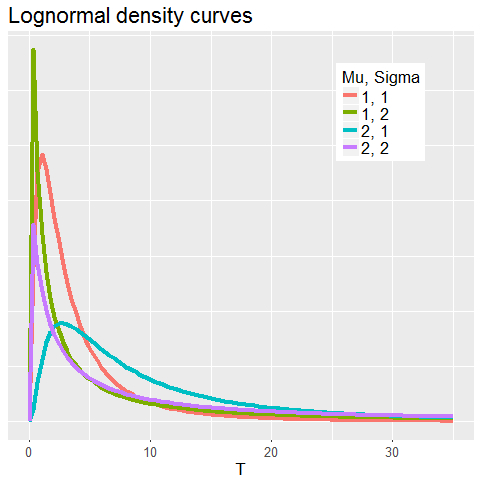
\includegraphics[width=0.35\textwidth]{Figures/lognormal.png}
%\end{frame}

\begin{frame}
\frametitle{PDF of Weibull random variable, $T$}
\begin{eqnarray}
f(t)=\frac{\beta t^{\beta-1}}{\lambda^{\beta}}e^{-(t/\lambda)^\beta},~t \geq 0,~\lambda > 0,~\beta > 0 \nonumber
\end{eqnarray}
%lambda = scale, beta = shape
\includegraphics[width=0.50\textwidth]{Figures/weibull.png}
\end{frame}

\begin{frame}
\frametitle{PDF of Exponential random variable, $T$}
\begin{eqnarray}
f(t)=(1/\lambda)e^{-t/\lambda},~t \geq 0,~\lambda > 0 \nonumber
\end{eqnarray}
% can also express in terms of lambda instead of 1/lambda (minitab uses lambda)
% the exponential distribution is a special case of the Weibull distribution for $\beta = 1$.
% lambda = scale parameter

\includegraphics[width=0.50\textwidth]{Figures/exponential.png}
\end{frame}

\begin{frame}
\frametitle{PDF of Lognormal random variable, $T$}
\begin{eqnarray}
f(t)=\frac{\exp\left[ -\frac{1}{2}\left(\frac{\ln(t)-\mu}{\sigma} \right)^2 \right]}{t(2\pi)^{1/2}\sigma}, ~t \geq 0,~\sigma > 0,~ -\infty < \mu < \infty \nonumber
\end{eqnarray}
%sigma = scale, mu=location
%\textbf{Note}: If $T$ follows a log-normal distribution, then $\ln (T)$ follows a normal distribution.
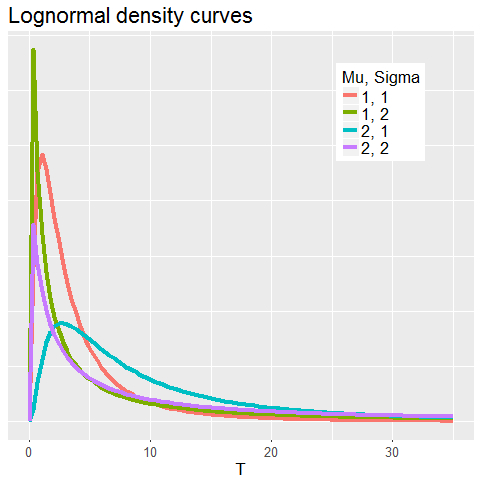
\includegraphics[width=0.50\textwidth]{Figures/lognormal.png}
\end{frame}

\begin{frame}
\frametitle{\grp}
\begin{columns}
\column{0.7\textwidth}
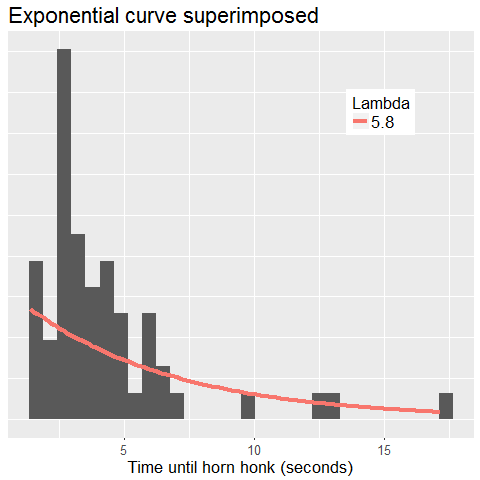
\includegraphics[width=1.0\textwidth]{Figures/motorists_exp.png}
\column{0.3\textwidth}
\begin{clicker}{Does the exponential density with $\lambda=5.8$ appear to provide a reasonable fit to the data?}
\begin{enumerate}
\item yes
\item no
\end{enumerate}
\end{clicker}
%no, this does not fit the data well
\end{columns}
\end{frame}


\begin{frame}
\frametitle{\grp}
\begin{columns}
\column{0.7\textwidth}
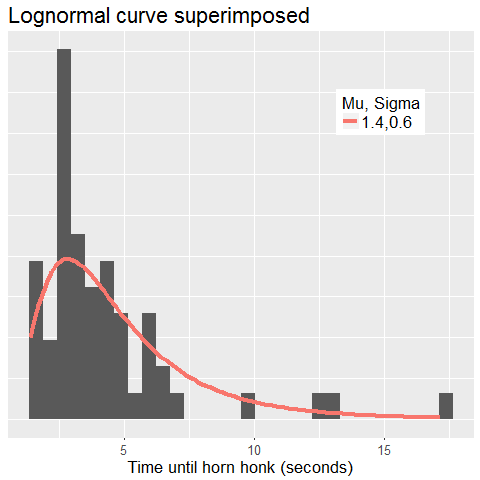
\includegraphics[width=1.0\textwidth]{Figures/motorists_lognormal.png}
\column{0.3\textwidth}
\begin{clicker}{Does the lognormal density with $\mu=1.4$ and $\sigma=0.6$ appear to provide a reasonable fit to the data?}
\begin{enumerate}
\item yes
\item no
\end{enumerate}
\end{clicker}
%yes, this provides a better fit than the exponential distribution
\end{columns}
\end{frame}


\begin{frame}
\frametitle{Cumulative distribution function}
%Once the probability distribution for $T$ has been determined, other models to characterize the time-to-event random variable can be derived.

The \emph{cumulative distribution function} (cdf) of a continuous time-to-event random variable $T$, $F(t)$, is the unconditional probability that an individual
experiences the event of interest before time $t$.
\begin{itemize}
\item $F(t)$ is defined as:
\item[]
\item[]
\item[]
%\begin{eqnarray}
%   \boxed{F(t)=P(T \leq t)= \int_{-\infty}^t f(y)dy} \nonumber
%\end{eqnarray}

\item Since the time-to-event random variable $T$ is non-negative, i.e. $t \geq 0$, $F(t)$ is given by:
\item[]
\item[]
\item[]
%\begin{center}
%$F(t)=P(T \leq t)=\int_{0}^t f(y)dy$
%\end{center}

%\item The height of $F(t)$ at point $t$ gives $P(T \leq t)$, and also corresponds to the area under the density curve $f(t)$ to the left of $t$.

%\item The cdf is a \textit{non-decreasing} function.
\end{itemize}

%pdf given by $f(t)=5e^{-5t}$, $t>0$.

\end{frame}

\begin{frame}
\frametitle{\grp}
What is $F(1)=Pr(T\leq 1$)?
%F(1)=0.841
\vskip10pt
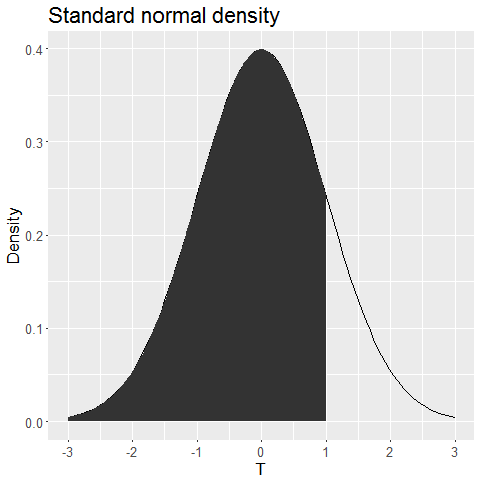
\includegraphics[width=0.48\textwidth]{Figures/shadednormalpdf.png}
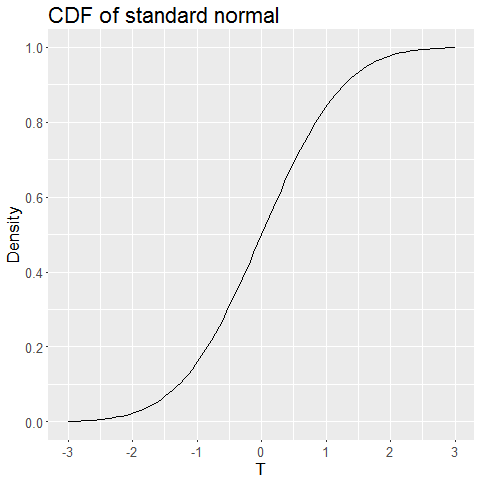
\includegraphics[width=0.48\textwidth]{Figures/normalcdf.png}
\end{frame}


\begin{frame}
\frametitle{\grp}
What is $F(5)=Pr(T\leq 5$)?
%F(1)=0.632
\vskip10pt
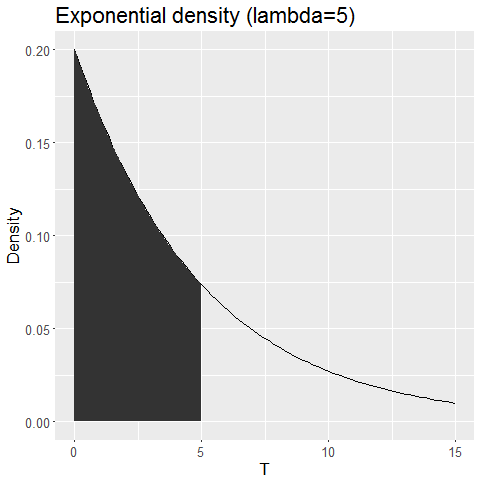
\includegraphics[width=0.48\textwidth]{Figures/shadedexppdf.png}
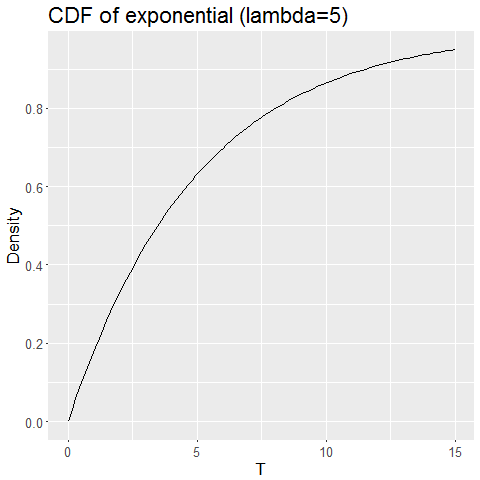
\includegraphics[width=0.48\textwidth]{Figures/expcdf.png}
\end{frame}

\begin{frame}
\frametitle{\grp}
Suppose the time until death (in days) for males with a particular type of inoperable lung cancer follows an exponential distribution with $\lambda = 125$.
\begin{enumerate}
\item Derive the cdf for the time-to-event random variable.
\end{enumerate}
\vskip 4in
\end{frame}

\begin{frame}
\frametitle{\grpc}
\begin{enumerate}
\setcounter{enumi}{1}
\item Use the cdf to find the probability that a randomly selected male with inoperable lung cancer will die in less than 75 days.
\item[]
\item[]
\item[]
\item[]
\item Use the cdf to find the probability that a randomly selected male with inoperable lung cancer will die between the 100th and 150th days.
\item[]
\item[]
\item[]
\item[]
\end{enumerate}
\end{frame}


\begin{frame}
\frametitle{Gompertz random variable}
%\item Not all probability distributions used to model time-to-event random variables are available in Minitab.
%\item Another probability distribution sometimes used to model time-to-event random variables is the Gompertz distribution.
If $T$ follows a Gompertz distribution with parameters $\theta>0$ and $\alpha>0$ then its pdf is given by:
\begin{eqnarray}
f(t)=\theta e^{\alpha t}\exp\left[\frac{\theta}{\alpha}\left(1-e^{\alpha t}\right)  \right],~t \geq 0 \nonumber
\end{eqnarray}
Suppose that the time to death in months for mice exposed to a high dose of radiation follows a Gompertz distribution with $\theta=.01$ and $\alpha = .25$
\begin{enumerate}
\item Derive the cdf for $T$.
\item Use the cdf to determine the probability that a randomly chosen mouse will die within 1 year of exposure.
\end{enumerate}
\vskip .8in
\end{frame}

\begin{frame}
\frametitle{Gompertz random variable, continued}
\end{frame}

\begin{frame}
\frametitle{Gompertz random variable, continued}
\end{frame}


\begin{frame}
\frametitle{Gompertz random variable, continued}
What is $F(12)=Pr(T\leq 12$)?
%F(1)=0.534
\vskip10pt
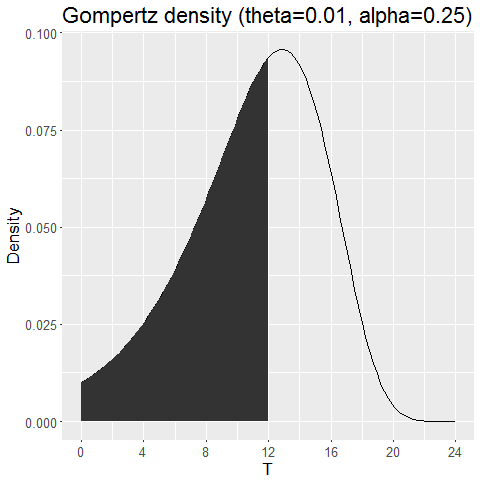
\includegraphics[width=0.48\textwidth]{Figures/shadedgompertzpdf.png}
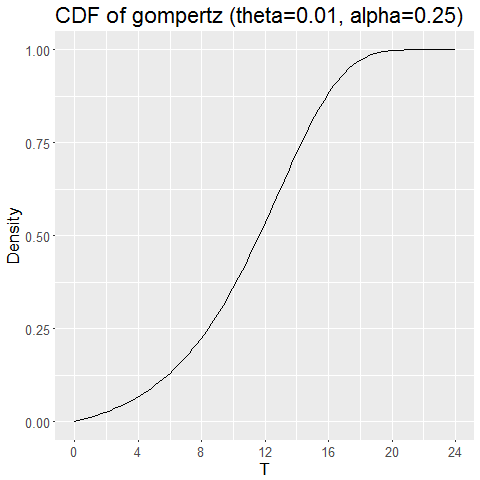
\includegraphics[width=0.48\textwidth]{Figures/gompertzcdf.png}
\end{frame}

\end{document}


